\section{Theorie}
\label{sec:Theorie}
Wenn Licht, welches als eine elektromagnetische Welle angesehen werden kann, schräg in ein anderes Medium eindringt, ändert der Lichtstrahl an der Grenzfläche
seie Richtung, da das Licht mit den Elektronen im Medium wechselwirkt und somit seine Ausbreitungsgeschwindigkeit verändert. Diese Brechung des Lichtes kann
quantitativ durch den Brechungsindex
\begin{equation}
n=\frac{v_1}{v_2}
\label{eq:1}
\end{equation}
beschrieben werden. Der Brechungsindex, welcher von den verschiedenen Geschwindigkeiten des Lichtes abhängt, wird mit Hilfe des Huygensschen Prinzips mit dem
Einfalls- und Brechungswinkel des Lichtstrahls verknüpft. Dieses besagt, dass jeder Punkt einer Welle als Zentrum einer neuen Kugelwelle angesehen werden kann.
Da der Lichtstrahl, wie in Abbildung \ref{fig:1} zu sehen, mit dem Winkel $\alpha$ gegen die Normale einfällt, trifft er zeitversetzt an den Punkten A und C
der Grenzfläche auf. Dadurch enstehen an dieser auch zeitversetzt neue Kugelwellen, welche sich schließlich zu einem, mit dem Winkel $\beta$ gegen die Normale
laufenden, Lichtstrahl überlagern.
\begin{figure}
  \centering
  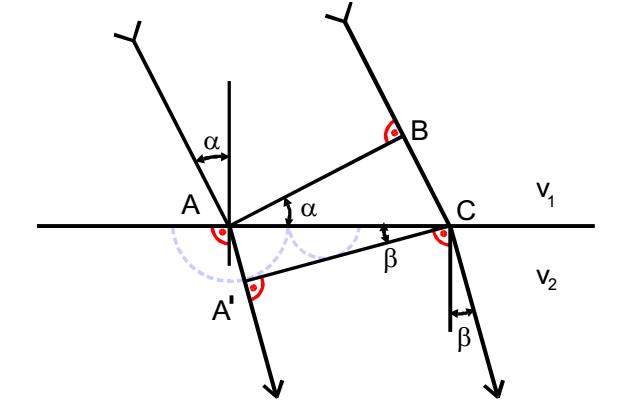
\includegraphics[scale=0.7]{fig1.png}
  \caption{Herleitung des Snelliusschen Brechungsgesetzes mit dem Huygensschen Prinzip. \cite{1}}
  \label{fig:1}
\end{figure}
Aus den in Abbildung \ref{fig:1} zu sehenden geometrischen Beziehungen lässt sich nun das Snelliussche Brechungsgesetz
\begin{equation}
\frac{sin(\alpha)}{sin(\beta)} = \frac{v_1}{v_2} = n
\label{eq:2}
\end{equation}
herleiten, welches durch Vergleich mit Gleichung (\ref{eq:1}) den Brechungsindex mit den Winkeln $\alpha$ und $\beta$ verknüpft.
Desweiteren ist die Ausbreitungsgeschwindigkeit und damit auch der Brechungsindex auch von den Welleneigenschaften  des Lichtes, wie der Frequenz $\omega$ und der
Wellenlänge $\lambda$, abhängig.
Diese sogenannte Dispersion wird durch die Dispersionskurve $n=f(\lambda)$ ausgedrückt.
Zur Herleitung dieser wird die Maxwellsche Theorie, sowie die Annahme, dass Materie aus Elektronen und Ionenrümpfen besteht, genutzt.
Das elektrische Wechselfeld des Lichts übt eine Kraft auf die Elektronen und Ionenrümpfen, welche Elementarladungen darstellen, aus, und lenkt
diese periodisch aus ihrer Ruhelage aus. So werden die Ladungen zu erzwungenen Schwingungen angeregt, wodurch auch Resonanzstellen auftreten, an welchen
die Energie des Lichts komplett absorbiert wird. Dieser Ansatz beschreibt die Wechselwirkung des Lichtes mit Materie nicht komplett, ist aber eine gute
Näherung für Wellenlängen im Bereich des sichtbaren Lichts, welche weit entfernt von den Resonanzstellen des Festkörpers sind. Nun wird die Differentialgleichung
für die erwzungenen Schwingungen durch Gleichsetzen der Coulombkraft, der Rückstellkraft und einer Reibungskraft im Festkörper aufgestellt und gelöst. Diese Lösung
wird nun umgeformt und stellt folgenden Zusammenhang zwischen Brechungsindex und Wellenlänge her:
\begin{equation}
  n^2 (\lambda) = 1 + \sum_h \frac{N_h \, {q_h}^2}{4 {\pi}^2 c^2 {\epsilon}_0 m_h} \, \frac{{\lambda}^2 {{\lambda}_h}^2}{{\lambda}^2 - {{\lambda}_h}^2} .
  \label{eq:3}
\end{equation}
Wird nun angenommen, dass es nur eine Resonanzstelle ${\lambda}_1$ gibt, lässt sich Gleichung (\ref{eq:3}) in zwei Potenzreihen entwickeln. So gilt für
$\lambda >> {\lambda}_1$:
\begin{equation}
n^2 (\lambda) = A_0 + \frac{A_2}{{\lambda}^2} + \frac{A_3}{{\lambda}^4} + \ldots \; \text{mit} \; A_0 , A_1 , A_2 \geq 0 .
\label{eq:4}
\end{equation}
Für $\lambda << {\lambda}_1$ gilt:
\begin{equation}
n^2 (\lambda) = 1 - {A'}_2 \, {\lambda}^2 - {A'}_4 \, {\lambda}^4 - \ldots \; \text{mit} \; {A'}_2 , {A'}_4 \geq 0 .
\label{eq:5}
\end{equation}
Die Vorfaktoren aus Gleichung (\ref{eq:3}) sind dabei in den Konstanten verarbeitet.
Die verschiedenen Dispersionskurven welche so entstehen sind in Abbildung \ref{fig:2} zu sehen.
\begin{figure}
  \centering
  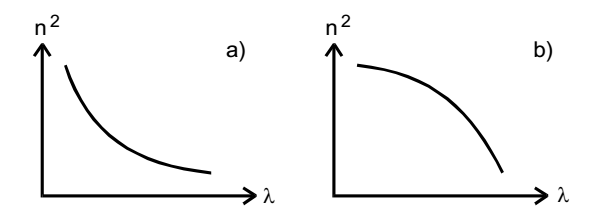
\includegraphics{fig2.png}
  \caption{Dispersionskurven: a) entspricht (\ref{eq:4}). b) entspricht (\ref{eq:5}). \cite{1}}
  \label{fig:2}
\end{figure}
